%!TEX root = ../tudkom_students__201804_v1.4.tex
\chapter{Evaluation}
\label{ch:evaluation}
%This chapter should describe how the evaluation of the implemented mechanism was done.
%1. Which evaluation method is used and why? Simulations, prototype?
%2. What is the goal of the evaluation? Comparison? Proof of concept?
%3. Wich metrics are used for characterizing the performance, costs, fairness, and efficiency of the system?
%4. What are the parameter settings used in the evaluation and why? If possible always justify why a certain threshold has been chose for a particular parameter.
%5. What is the outcome of the evaluation?
% 5-10 pages

\section{Ziele}
Mit dem Wearable werden einige Tests mit Blick auf die in der Einleitung \ref{ch:aims} aufgestellten Ziele gemacht.
Die Austauschbarkeit der Protokolle und Komponenten wird durch die Implementierung erreicht.
Insbesondere die Trennung des Codes von Endgerät, MCU, IMU und dem Protokoll zwischen MCU und IMU tragen dazu bei.
Ob die Größe und das Gewicht ausreichend gering sind, ist vom Anwendungsfall abhängig.
Bei dem Wearable sind sie stark von der Knopfzelle geprägt.
Es wurde die etwa 2.36 cm\textsuperscript{3} große CR2450 statt der etwa 1.01 cm\textsuperscript{3} großen CR2032 gewählt um die 2.7-fache Energiekapazität zu erhalten.
Um die Entscheidung zu ändern, muss nur das Platinenlayout überarbeitet werden während das Schaltbild und der Code übernommen werden können.
Ob die Kapazität der Knopfzellen überhaupt anwendungstauglich ist, soll in den Tests zum Energieverbrauch ermittelt werden.
Dafür sollen verschiedene Parameter geändert werden und der Einfluss auf die Energieaufnahme gemessen und die Auswirkungen auf die Datenübertragung evaluiert werden.
Bei der Datenübertragung kann zum Einen die Menge der Sensordaten pro Sekunde gemessen werden.
Zum Anderen kann geprüft werden, wie regelmäßig die Sensordaten beim Endgerät ankommen.\\
Es wurde die Energieaufnahme verglichen in den Szenarien Prototyp mit LSM6DSL IMU vs Wearable und LSM6DSL IMU vs BMI160 IMU auf dem Prototypen.
Der Prototyp besteht aus dem nRF52 DK und dem STEVAL-MKI178V2 bzw. BMI160 Shuttle Board.
Die Auswirkungen auf die Energieaufnahme und der Datenübertragung wurden auf dem Wearable bei einer Änderung der Größe des TX-Buffers, MTU-Größe, Connection Interval, SPI-Frequenz und Sensordatenrate erfasst.

\section{Methoden}
Zur Messung der Datenrate wird auf dem Smartphone angezeigt, wie viele Datenpakete in einer Sekunde ankommen.
Um die Regelmäßigkeit zu vergleichen wird die Datenrate pro Sekunde über einen Zeitraum aufgenommen und die Formel \ref{eq:standardabweichung} für die Standardabweichung mit dem unverzerrten Schätzer angewandt.
\begin{equation}
  \label{eq:standardabweichung}
	s = \sqrt{\cfrac{1}{n-1}\sum_{i=1}^{n} (x_{i}-\overline{x})^{2}}\text{, mit n = Anzahl der Werte und $\overline{x}$ = eingestellte Sensordatenrate}
\end{equation}
Die Standardabweichung wird wiederum in einem anderem Graphen auf dem Smartphone aufgezeichnet, sobald Daten von mindestens 30 Sekunden vorliegen.\\
Um die Stromaufnahme zu messen, wird das ohmsche Gesetz $I = \cfrac{U}{R}$ benötigt.
Wird ein Widerstand in Reihe mit der Spannungsversorgung des Wearables geschaltet, ist ein Spannungsabfall um den Widerstand zu messen.
Da man den Wert des Widerstandes kennt und den Spannungsabfall mit einem Oszilloskop messen kann, lässt sich mit der Formel der Strom berechnen.
Bei der Wahl des Widerstandes gilt: Je größer der Widerstand, desto mehr Spannung fällt ab.
Ist die Spannung zu klein, lässt sie sich nicht genau messen.
Ist die Spannung zu groß, bleibt nicht genug Spannung für das Wearable übrig.
Um den Strom in verschiedenen Messbereichen berechnen zu können, werden die passenden Widerstände benötigt.
Um den Widerstand anpassen zu können, wurde eine Lochrasterplatine, die in Abbildung \ref{fig:messplatine} zu sehen ist, mit Widerständen bestückt, die mit Steckbrücken in den Stromkreis integriert werden können.
\begin{figure}[hbtp]
	\centering
	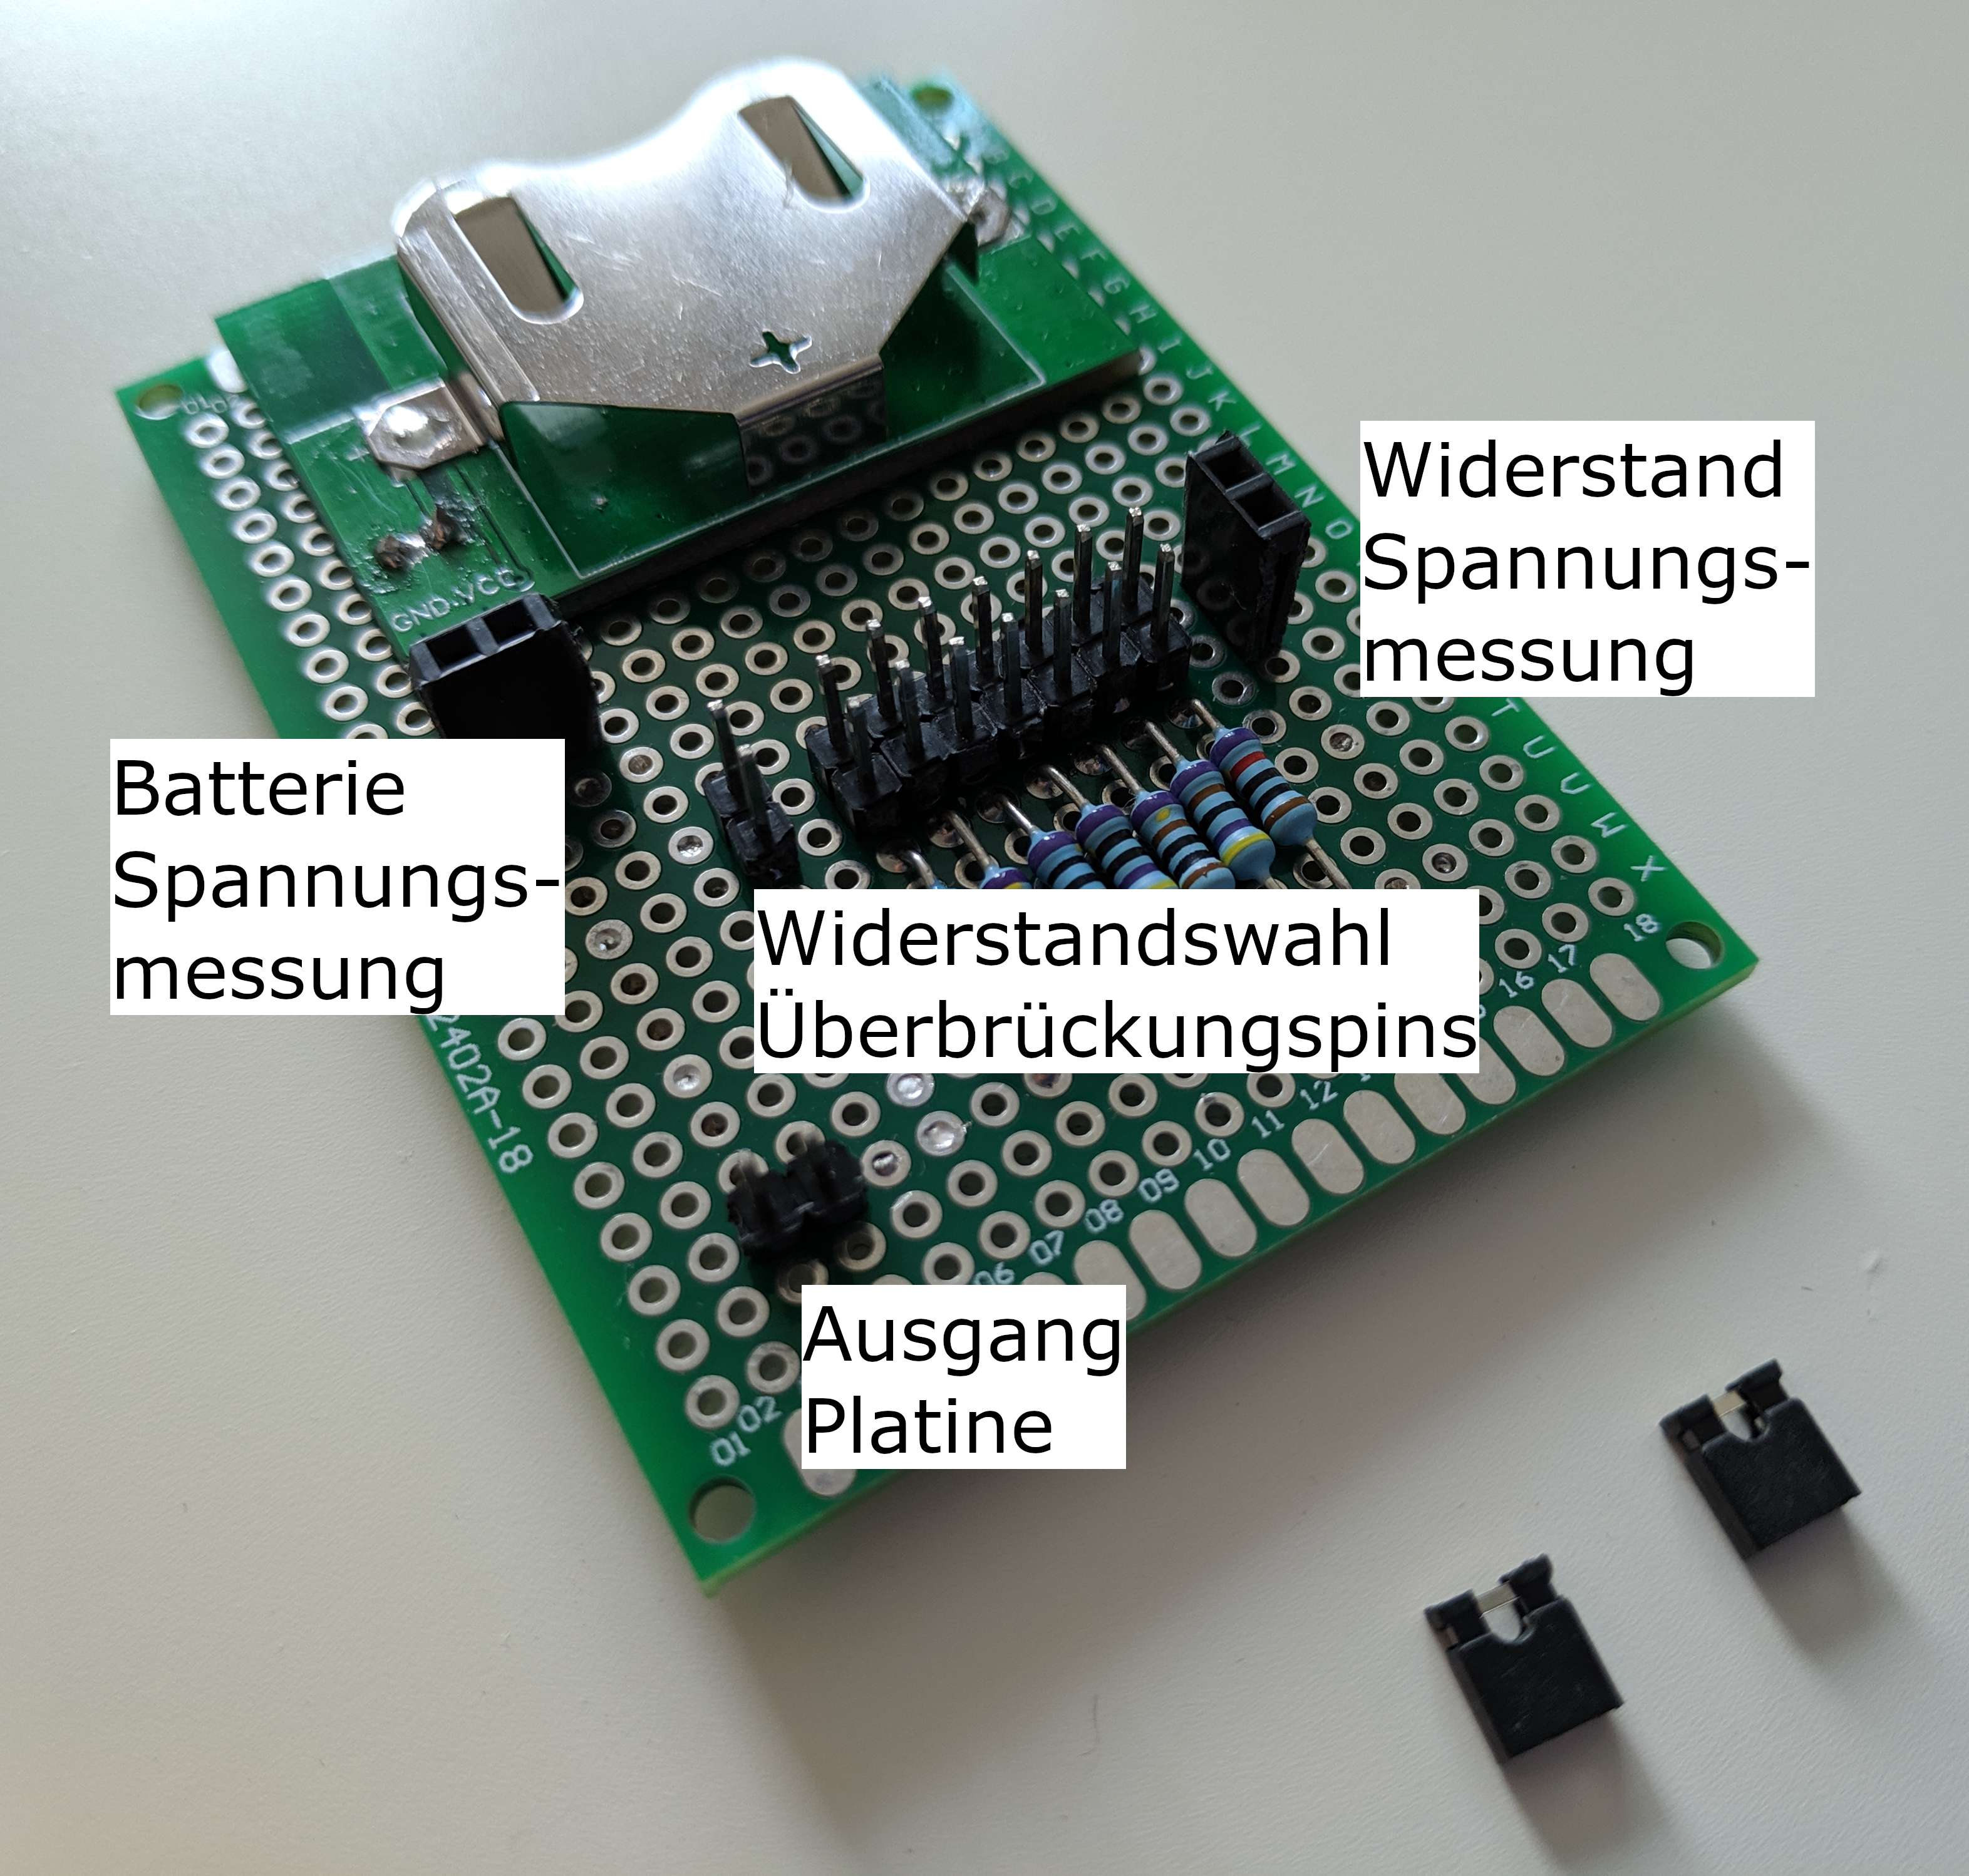
\includegraphics[width=0.45\linewidth]{res/messplatine.jpg}
	\caption{Messplatine}
	\label{fig:messplatine}
\end{figure}
Die Widerstände haben eine Toleranz von 0.1 \% und Werte von 0, 10, 47, 100, 470, 1000, 4700 und 10000 Ohm.\\
Das Oszilloskop ist ein Picoscope 5444B.
Der Spannungsabfall wurde mit einer Frequenz 2 GHz gemessen.
Technisch bedingt kann der Mittelwert nur über 5 Sekunden automatisch gebildet werden.
Deshalb wurde jeder Test 6 Mal abgeschlossen.
Das Offset wurde vor dem Test kalibriert.
Als Spannungsquelle wurde eine neue CR2450 Knopfzelle und ein Voltcraft Model 2256 Netzgerät genutzt.
Da das Netzteil bei zu geringer Last keine stabile Spannung erzeugen kann, wurde dem Testobjekt ein Widerstand von 58.75 Ohm parallel geschaltet.
Das Netzteil wurde so eingestellt, dass am Testobjekt eine Spannung zwischen 2.95 und 3 V anliegt.
Vor jeder Testreihe wurde die Spannung am Netzteil nachjustiert oder die Spannung der Batterie notiert.\\
Beim Prototypen wurde die Diode zum Verpolungsschutz mit SB12 überbrückt, wie in der Anleitung zum nRF52 DK angegeben \cite{site_nrf52dk}.
Der Spannungsabfall wurde direkt an der Spannungsquelle gemessen und nicht an den Pins 'nRF current measurement'.
Nach dem Schaltbild von Figur 8 in \cite{site_nrf52dk} ließe sich sonst nur der Strom, der von der MCU aufgenommen wird, messen und der Verbrauch der IMU wäre nicht mit eingegangen.
Der Hinweis über Figur 8 besagt, dass die MCU bei der verwendeten Methode wegen der Reset-Funktion 20 $\mu$A mehr Strom verbraucht.
Da der Reset-Knopf erst eine Funktion zeigt, wenn auch SB10 überbrückt wird, kann erst mit den vorliegenden Ergebnissen eine Aussage getroffen werden, ob sich der Prototyp dahingehend vom Wearable unterschiedet.

\section{Ergebnisse}
Der erste Teil der Tabellen listet die Rahmenbedingungen für die Tests auf.
Die Zeilen der Daten sind die Beschreibung des Testfalls, der maximale gemessene Spannungsspitze und der Durchschnitt der sechs Testfälle.
Die Spalten der Daten sind: Testnummer, gemessene Spannung und resultierender Strom.

\subsubsection{Energieaufnahme mit LSM6DSL: Prototyp vs Wearable}
\begin{minipage}{\linewidth}
	\captionof{table}{Prototyp vs Wearable}
	\label{tab:aaaaaaaaaaaaaaaa}
	\begin{tabularx}{\linewidth}{|l|l|X|}
		Widerstand & \multicolumn{2}{l|}{10 Ohm}\\
    SPI-Frequenz & \multicolumn{2}{l|}{4 MHz}\\
    MTU-Größe & \multicolumn{2}{l|}{23 Byte}\\
    TX-Buffer & \multicolumn{2}{l|}{10 Einträge}\\
    Spannungsquelle & \multicolumn{2}{l|}{Netzteil}\\
    MCU & \multicolumn{2}{l|}{Wearable und Prototyp}\\
    IMU & \multicolumn{2}{l|}{LSM6DSL und BMI160}\\
    Sensordatenrate & \multicolumn{2}{l|}{200 Hz und 0 Hz}\\
    Connection Interval & \multicolumn{2}{l|}{High}\\
    \hline
    \multicolumn{3}{c}{Wearable LSM6DSL 200 Hz}\\
    Spitze & 196 mV & mA\\
    AVG & 24.555 mV & mA\\
    \hline
    \multicolumn{3}{c}{Wearable LSM6DSL 0 Hz}\\
    Spitze & 138 mV & mA\\
    AVG & 3.55 mV & mA\\
    \hline
    \multicolumn{3}{|c|}{Prototyp LSM6DSL 200 Hz}\\
    Spitze & 180 mV & 18 mA\\
    AVG & 29.455 mV & mA\\
    \hline
    \multicolumn{3}{|c|}{Prototyp LSM6DSL 0 Hz}\\
    Spitze & 127 mV & mA\\
    AVG & 10.153 mV & mA\\
    \hline
    \multicolumn{3}{|c|}{Prototyp BMI160 200 Hz}\\
    Spitze & 186 mV & mA\\
    AVG & 34.958 mV & mA\\
    \hline
    \multicolumn{3}{|c|}{Prototyp BMI160 0 Hz}\\
    Spitze & 122 mV & mA\\
    AVG & 10.031 mV & mA\\
  \end{tabularx}
\end{minipage}\\\\

\subsubsection{Änderung von TX-Buffer}
\begin{minipage}{\linewidth}
	\captionof{table}{Prototyp vs Wearable}
	\label{tab:aaaaaaaaaaaaaaaa}
	\begin{tabularx}{\linewidth}{|l|l|X|}
		Widerstand & \multicolumn{2}{l|}{47 Ohm}\\
    SPI-Frequenz & \multicolumn{2}{l|}{1 MHz}\\
    MTU-Größe & \multicolumn{2}{l|}{23 Byte}\\
    TX-Buffer & \multicolumn{2}{l|}{1, 50 und 300 Einträge}\\
    Algorithmus & \multicolumn{2}{l|}{An und Aus}\\
    Spannungsquelle & \multicolumn{2}{l|}{Batterie 3.044 V}\\
    MCU & \multicolumn{2}{l|}{Wearable}\\
    IMU & \multicolumn{2}{l|}{LSM6DSL}\\
    Sensordatenrate & \multicolumn{2}{l|}{200 Hz}\\
    Connection Interval & \multicolumn{2}{l|}{High}\\
    \hline
    \multicolumn{3}{|c|}{TX1 Algo=An}\\
    Spitze & 794 mV & mA\\
    AVG & 125.267 mV & mA\\
    \hline
    \multicolumn{3}{|c|}{TX50 Algo=An}\\
    Spitze & 794 mV & mA\\
    AVG & 126.2 mV & mA\\
    \hline
    \multicolumn{3}{|c|}{TX300 Algo=An}\\
    Spitze & 794 mV & mA\\
    AVG & 126.217 mV & mA\\
    \hline
    \multicolumn{3}{|c|}{TX1 Algo=Aus}\\
    Spitze & 794 mV & mA\\
    AVG & 125.317 mV & mA\\
    \hline
    \multicolumn{3}{|c|}{TX50 Algo=Aus}\\
    Spitze & 794 mV & mA\\
    AVG & 125.883 mV & mA\\
    \hline
    \multicolumn{3}{|c|}{TX300 Algo=Aus}\\
    Spitze & 794 mV & mA\\
    AVG & 125.9 mV & mA\\
  \end{tabularx}
\end{minipage}\\\\

\subsubsection{Änderung von MTU-Größe}
\begin{minipage}{\linewidth}
	\captionof{table}{Prototyp vs Wearable}
	\label{tab:aaaaaaaaaaaaaaaa}
	\begin{tabularx}{\linewidth}{|l|l|X|}
		Widerstand & \multicolumn{2}{l|}{47 Ohm}\\
    SPI-Frequenz & \multicolumn{2}{l|}{1 MHz}\\
    MTU-Größe & \multicolumn{2}{l|}{150 und 517 Byte}\\
    TX-Buffer & \multicolumn{2}{l|}{10 und 50 Einträge}\\
    Spannungsquelle & \multicolumn{2}{l|}{Batterie 3.044 V}\\
    MCU & \multicolumn{2}{l|}{Wearable}\\
    IMU & \multicolumn{2}{l|}{LSM6DSL}\\
    Sensordatenrate & \multicolumn{2}{l|}{200 Hz}\\
    Connection Interval & \multicolumn{2}{l|}{High}\\
    \hline
    \multicolumn{3}{|c|}{MTU150 TX10}\\
    Spitze & 794 mV & mA\\
    AVG & 125.8 mV & mA\\
    \hline
    \multicolumn{3}{|c|}{MTU517 TX10}\\
    Spitze & 794 mV & mA\\
    AVG & 126.1 mV & mA\\
    \hline
    \multicolumn{3}{|c|}{MTU150 TX50}\\
    Spitze & 794 mV & mA\\
    AVG & 125.783 mV & mA\\
  \end{tabularx}
\end{minipage}\\\\

\subsubsection{Änderung von SPI-Frequenz}
\begin{minipage}{\linewidth}
	\captionof{table}{Prototyp vs Wearable}
	\label{tab:aaaaaaaaaaaaaaaa}
	\begin{tabularx}{\linewidth}{|l|l|X|}
		Widerstand & \multicolumn{2}{l|}{47 Ohm}\\
    SPI-Frequenz & \multicolumn{2}{l|}{125 kHz, 1 MHz, 8 MHz}\\
    MTU-Größe & \multicolumn{2}{l|}{35 Byte}\\
    TX-Buffer & \multicolumn{2}{l|}{10 Einträge}\\
    Spannungsquelle & \multicolumn{2}{l|}{Batterie 3.044 V}\\
    MCU & \multicolumn{2}{l|}{Wearable}\\
    IMU & \multicolumn{2}{l|}{LSM6DSL}\\
    Sensordatenrate & \multicolumn{2}{l|}{400 Hz}\\
    Connection Interval & \multicolumn{2}{l|}{High}\\
    \hline
    \multicolumn{3}{|c|}{125kHz}\\
    Spitze & 794 mV & mA\\
    AVG & 294.95 mV & mA\\
    \hline
    \multicolumn{3}{|c|}{1MHz}\\
    Spitze & 794 mV & mA\\
    AVG & 187.817 mV & mA\\
    \hline
    \multicolumn{3}{|c|}{8MHz}\\
    Spitze & 794 mV & mA\\
    AVG & 173.233 mV & mA\\
  \end{tabularx}
\end{minipage}\\\\

\subsubsection{Änderung von Connection Interval}
\begin{minipage}{\linewidth}
	\captionof{table}{Prototyp vs Wearable}
	\label{tab:aaaaaaaaaaaaaaaa}
	\begin{tabularx}{\linewidth}{|l|l|X|}
		Widerstand & \multicolumn{2}{l|}{47 Ohm}\\
    SPI-Frequenz & \multicolumn{2}{l|}{4 MHz}\\
    MTU-Größe & \multicolumn{2}{l|}{35 Byte}\\
    TX-Buffer & \multicolumn{2}{l|}{10 Einträge}\\
    Spannungsquelle & \multicolumn{2}{l|}{Batterie 2.991 V}\\
    MCU & \multicolumn{2}{l|}{Wearable}\\
    IMU & \multicolumn{2}{l|}{LSM6DSL}\\
    Sensordatenrate & \multicolumn{2}{l|}{0 und 100 Hz}\\
    Connection Interval & \multicolumn{2}{l|}{Low, Balance, High}\\
    \hline
    \multicolumn{3}{|c|}{Low 0Hz}\\
    Spitze & 625 mV & mA\\
    AVG & 22.715 mV & mA\\
    \hline
    \multicolumn{3}{|c|}{Balance 0Hz}\\
    Spitze & 614 mV & mA\\
    AVG & 27.27 mV & mA\\
    \hline
    \multicolumn{3}{|c|}{High 0Hz}\\
    Spitze & 572 mV & mA\\
    AVG & 36.652 mV & mA\\
    \hline
    \multicolumn{3}{|c|}{Low 100Hz}\\
    Spitze & 794 mV & mA\\
    AVG & 83.443 mV & mA\\
    \hline
    \multicolumn{3}{|c|}{Balance 100Hz}\\
    Spitze & 794 mV & mA\\
    AVG & 86.188 mV & mA\\
    \hline
    \multicolumn{3}{|c|}{High 100Hz}\\
    Spitze & 794 mV & mA\\
    AVG & 94.575 mV & mA\\
  \end{tabularx}
\end{minipage}\\\\

\subsubsection{Änderung von Sensordatenrate}
\begin{minipage}{\linewidth}
	\captionof{table}{Prototyp vs Wearable}
	\label{tab:aaaaaaaaaaaaaaaa}
	\begin{tabularx}{\linewidth}{|l|l|X|}
		Widerstand & \multicolumn{2}{l|}{47 Ohm}\\
    SPI-Frequenz & \multicolumn{2}{l|}{4 MHz}\\
    MTU-Größe & \multicolumn{2}{l|}{35 Byte}\\
    TX-Buffer & \multicolumn{2}{l|}{10 Einträge}\\
    Spannungsquelle & \multicolumn{2}{l|}{Batterie 2.991 V}\\
    MCU & \multicolumn{2}{l|}{Wearable}\\
    IMU & \multicolumn{2}{l|}{LSM6DSL}\\
    Sensordatenrate & \multicolumn{2}{l|}{25, 50, 100, 200, 400 und 800 Hz}\\
    Connection Interval & \multicolumn{2}{l|}{High}\\
    \hline
    \multicolumn{3}{|c|}{25Hz}\\
    Spitze & 762 mV & mA\\
    AVG & 78.043 mV & mA\\
    \hline
    \multicolumn{3}{|c|}{50Hz}\\
    Spitze & 784 mV & mA\\
    AVG & 83.378 mV & mA\\
    \hline
    \multicolumn{3}{|c|}{100Hz}\\
    Spitze & 794 mV & mA\\
    AVG & 98.362 mV & mA\\
    \hline
    \multicolumn{3}{|c|}{200Hz}\\
    Spitze & 794 mV & mA\\
    AVG & 125.233 mV & mA\\
    \hline
    \multicolumn{3}{|c|}{400Hz}\\
    Spitze & 794 mV & mA\\
    AVG & 180.817 mV & mA\\
    \hline
    \multicolumn{3}{|c|}{800Hz}\\
    Spitze & 805 mV & mA\\
    AVG & 286.167 mV & mA\\
  \end{tabularx}
\end{minipage}\\\\

\subsubsection{Ältere Ergebnisse}
\begin{minipage}{\linewidth}
	\captionof{table}{Prototyp vs Wearable}
	\label{tab:aaaaaaaaaaaaaaaa}
	\begin{tabularx}{\linewidth}{|l|l|X|}
		Widerstand & \multicolumn{2}{l|}{47 und 10000 Ohm}\\
    SPI-Frequenz & \multicolumn{2}{l|}{4 MHz}\\
    MTU-Größe & \multicolumn{2}{l|}{35 Byte}\\
    TX-Buffer & \multicolumn{2}{l|}{10 Einträge}\\
    Spannungsquelle & \multicolumn{2}{l|}{Batterie 2.875 - 2.916 V}\\
    MCU & \multicolumn{2}{l|}{Wearable}\\
    IMU & \multicolumn{2}{l|}{LSM6DSL}\\
    Sensordatenrate & \multicolumn{2}{l|}{25, 50, 100, 200, 400 und 800 Hz}\\
    Connection Interval & \multicolumn{2}{l|}{High}\\
    \hline
    \multicolumn{3}{|c|}{25Hz}\\
    Spitze & 762 mV & mA\\
    AVG & 78.043 mV & mA\\
    \hline
    \multicolumn{3}{|c|}{50Hz}\\
    Spitze & 784 mV & mA\\
    AVG & 83.378 mV & mA\\
    \hline
    \multicolumn{3}{|c|}{100Hz}\\
    Spitze & 794 mV & mA\\
    AVG & 98.362 mV & mA\\
    \hline
    \multicolumn{3}{|c|}{200Hz}\\
    Spitze & 794 mV & mA\\
    AVG & 125.233 mV & mA\\
    \hline
    \multicolumn{3}{|c|}{400Hz}\\
    Spitze & 794 mV & mA\\
    AVG & 180.817 mV & mA\\
    \hline
    \multicolumn{3}{|c|}{800Hz}\\
    Spitze & 805 mV & mA\\
    AVG & 286.167 mV & mA\\
  \end{tabularx}
\end{minipage}\\\\



\section{Analysis of Results}
\begin{figure}[hbtp]
	\centering
	\includegraphics[width=0.5\linewidth]{res/android.jpg}
	\caption{Screenshot der Graphen von Datenrate und Standardabweichung}
	\label{fig:android}
\end{figure}
